
\documentclass[a4paper]{article}
\usepackage{graphicx}     % Om figuren te laten zien
\usepackage[fleqn]{amsmath} % Voor wiskundige symbolen
\usepackage{hyperref}     % Voor externe links. 
\usepackage{chemfig}
\usepackage{pdfpages}
\begin{document}
	
\title{Report Software Design}

\author{R. de Berg, J. Schoppink, N. Zankavets}

\date{\today}

\maketitle
The idea of the software design project was to create an interface from which the whole box could be operated. Inside the box there are devices that can acquire data, such as several Arduinos to measure for temperature, vibration control, and humidity. There is also an Analog Discovery 2 by Digilent for the Cavendish experiment. \\\\
\indent Of course it is possible to run four or five different programs on a single laptop and control the box from there. Especially in the case of the Analog Discovery 2, where the manufacturer has already provided a program. However, it would be significantly easier and more structured to have all of it present in a single program. That is why we made the Beautiful Interface of Magic Box Operations. Another advantage of building your own program, is that it will not be cluttered with features that you will not need.\\\\
\indent When you run the python script that opens this program, the first thing you will see is a start screen. This is shown in figure \ref{fig1}. This purpose of this screen is to make sure you have opened the correct program and also includes a bit of marketing and product promotion in the form of a logo. This enhances the product recognition among the users of the program. \\\\

\begin{figure}[]
	\centering
	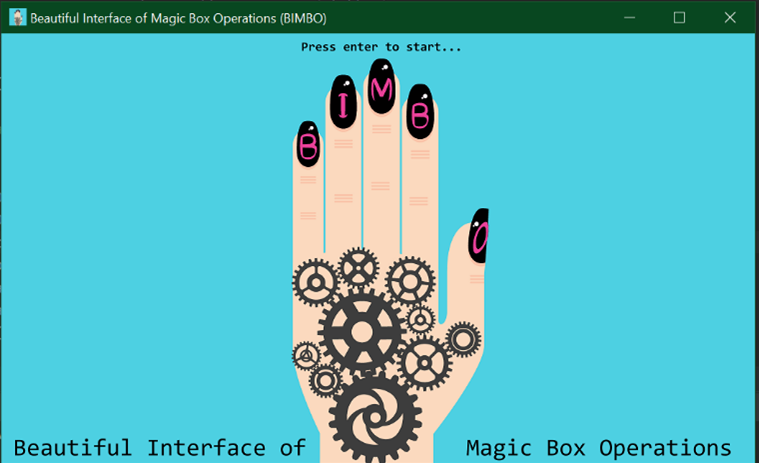
\includegraphics[width=0.7 \textwidth]{startscreen.png}
	\caption{\label{fig1} The start screen of the program.}
\end{figure}

\indent After pressing enter the real program will open. This is an interface where you can navigate to different devices using the tabs in the top-left. In figure \ref{fig1} the first tab is shown. This tab gives an overview of the other tabs. It has not yet been implemented. This will be done to make it easy to set up your experiment. With a quick glance at the overview screen you can make sure your devices are set up correctly and displaying values.\\\\

\begin{figure}[h]
	\centering
	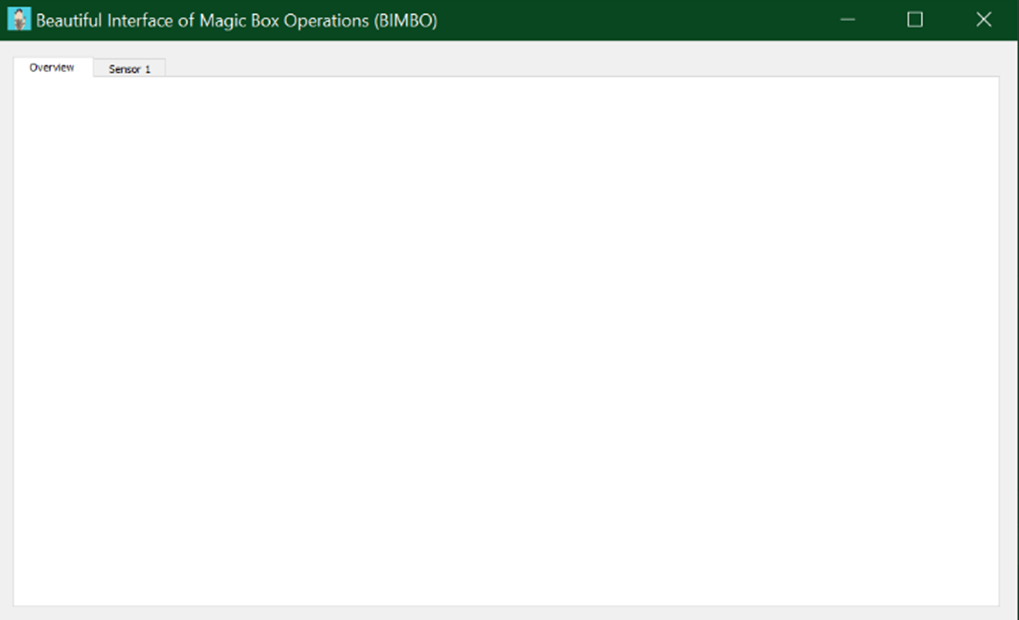
\includegraphics[width=0.7 \textwidth]{overview.png}
	\caption{\label{fig2} The overview window.}
\end{figure}

\indent In figure \ref{fig3} an example control window is shown. In this tab, the user will be able to control the Analog Discovery 2 by setting the output voltages for channel 1 and 2 on the left. Once start is pressed the monitor windows on the right start showing the current input voltages for channels 1 and 2.\\\\ 

\begin{figure}[h]
	\centering
	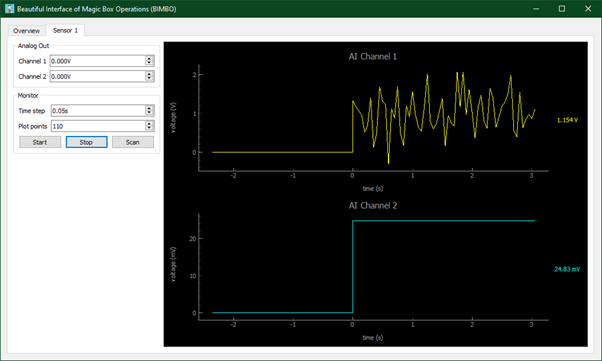
\includegraphics[width=0.7 \textwidth]{tab1.png}
	\caption{\label{fig3} The first tab with an example display.}
\end{figure}

\indent A scan button was introduced in order to be able to save the data. When this button is pressed, a new window is opened where you can save your data after scanning a certain voltage or time range. In figure \ref{fig5} the scan screen is shown. As can be seen, this is an external window. You are thus still able to navigate between the different tabs in the main program.\\\\
\indent We believe that in the context of the box, it makes a lot of sense to write your own program. One of the main features of the box it its modular nature. Once a different experiment is added to the box, it will be quite easy to add another tab to the BIMBO program. Of course, users of the box are always free use their own programs and use BIMBO merely as control program for the box but not their experiment.
\begin{figure}[h]
	\centering
	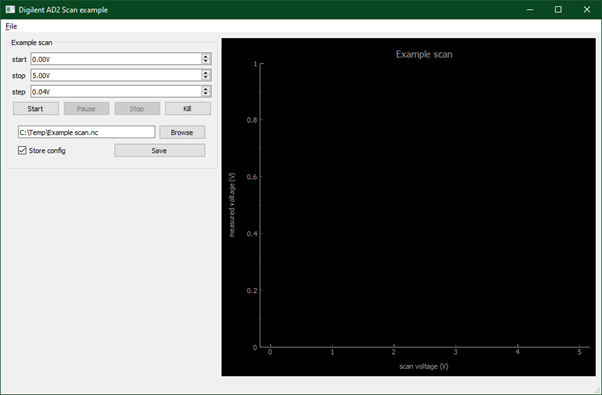
\includegraphics[width=0.7 \textwidth]{scanwindow.png}
	\caption{\label{fig5} The scan window.}
\end{figure}


\end{document}






